% Options for packages loaded elsewhere
\PassOptionsToPackage{unicode}{hyperref}
\PassOptionsToPackage{hyphens}{url}
%
\documentclass[
]{article}
\usepackage{lmodern}
\usepackage{amssymb,amsmath}
\usepackage{ifxetex,ifluatex}
\ifnum 0\ifxetex 1\fi\ifluatex 1\fi=0 % if pdftex
  \usepackage[T1]{fontenc}
  \usepackage[utf8]{inputenc}
  \usepackage{textcomp} % provide euro and other symbols
\else % if luatex or xetex
  \usepackage{unicode-math}
  \defaultfontfeatures{Scale=MatchLowercase}
  \defaultfontfeatures[\rmfamily]{Ligatures=TeX,Scale=1}
\fi
% Use upquote if available, for straight quotes in verbatim environments
\IfFileExists{upquote.sty}{\usepackage{upquote}}{}
\IfFileExists{microtype.sty}{% use microtype if available
  \usepackage[]{microtype}
  \UseMicrotypeSet[protrusion]{basicmath} % disable protrusion for tt fonts
}{}
\makeatletter
\@ifundefined{KOMAClassName}{% if non-KOMA class
  \IfFileExists{parskip.sty}{%
    \usepackage{parskip}
  }{% else
    \setlength{\parindent}{0pt}
    \setlength{\parskip}{6pt plus 2pt minus 1pt}}
}{% if KOMA class
  \KOMAoptions{parskip=half}}
\makeatother
\usepackage{xcolor}
\IfFileExists{xurl.sty}{\usepackage{xurl}}{} % add URL line breaks if available
\IfFileExists{bookmark.sty}{\usepackage{bookmark}}{\usepackage{hyperref}}
\hypersetup{
  pdftitle={Worksheet 2; Chi Distribution},
  hidelinks,
  pdfcreator={LaTeX via pandoc}}
\urlstyle{same} % disable monospaced font for URLs
\usepackage[margin=1in]{geometry}
\usepackage{color}
\usepackage{fancyvrb}
\newcommand{\VerbBar}{|}
\newcommand{\VERB}{\Verb[commandchars=\\\{\}]}
\DefineVerbatimEnvironment{Highlighting}{Verbatim}{commandchars=\\\{\}}
% Add ',fontsize=\small' for more characters per line
\usepackage{framed}
\definecolor{shadecolor}{RGB}{248,248,248}
\newenvironment{Shaded}{\begin{snugshade}}{\end{snugshade}}
\newcommand{\AlertTok}[1]{\textcolor[rgb]{0.94,0.16,0.16}{#1}}
\newcommand{\AnnotationTok}[1]{\textcolor[rgb]{0.56,0.35,0.01}{\textbf{\textit{#1}}}}
\newcommand{\AttributeTok}[1]{\textcolor[rgb]{0.77,0.63,0.00}{#1}}
\newcommand{\BaseNTok}[1]{\textcolor[rgb]{0.00,0.00,0.81}{#1}}
\newcommand{\BuiltInTok}[1]{#1}
\newcommand{\CharTok}[1]{\textcolor[rgb]{0.31,0.60,0.02}{#1}}
\newcommand{\CommentTok}[1]{\textcolor[rgb]{0.56,0.35,0.01}{\textit{#1}}}
\newcommand{\CommentVarTok}[1]{\textcolor[rgb]{0.56,0.35,0.01}{\textbf{\textit{#1}}}}
\newcommand{\ConstantTok}[1]{\textcolor[rgb]{0.00,0.00,0.00}{#1}}
\newcommand{\ControlFlowTok}[1]{\textcolor[rgb]{0.13,0.29,0.53}{\textbf{#1}}}
\newcommand{\DataTypeTok}[1]{\textcolor[rgb]{0.13,0.29,0.53}{#1}}
\newcommand{\DecValTok}[1]{\textcolor[rgb]{0.00,0.00,0.81}{#1}}
\newcommand{\DocumentationTok}[1]{\textcolor[rgb]{0.56,0.35,0.01}{\textbf{\textit{#1}}}}
\newcommand{\ErrorTok}[1]{\textcolor[rgb]{0.64,0.00,0.00}{\textbf{#1}}}
\newcommand{\ExtensionTok}[1]{#1}
\newcommand{\FloatTok}[1]{\textcolor[rgb]{0.00,0.00,0.81}{#1}}
\newcommand{\FunctionTok}[1]{\textcolor[rgb]{0.00,0.00,0.00}{#1}}
\newcommand{\ImportTok}[1]{#1}
\newcommand{\InformationTok}[1]{\textcolor[rgb]{0.56,0.35,0.01}{\textbf{\textit{#1}}}}
\newcommand{\KeywordTok}[1]{\textcolor[rgb]{0.13,0.29,0.53}{\textbf{#1}}}
\newcommand{\NormalTok}[1]{#1}
\newcommand{\OperatorTok}[1]{\textcolor[rgb]{0.81,0.36,0.00}{\textbf{#1}}}
\newcommand{\OtherTok}[1]{\textcolor[rgb]{0.56,0.35,0.01}{#1}}
\newcommand{\PreprocessorTok}[1]{\textcolor[rgb]{0.56,0.35,0.01}{\textit{#1}}}
\newcommand{\RegionMarkerTok}[1]{#1}
\newcommand{\SpecialCharTok}[1]{\textcolor[rgb]{0.00,0.00,0.00}{#1}}
\newcommand{\SpecialStringTok}[1]{\textcolor[rgb]{0.31,0.60,0.02}{#1}}
\newcommand{\StringTok}[1]{\textcolor[rgb]{0.31,0.60,0.02}{#1}}
\newcommand{\VariableTok}[1]{\textcolor[rgb]{0.00,0.00,0.00}{#1}}
\newcommand{\VerbatimStringTok}[1]{\textcolor[rgb]{0.31,0.60,0.02}{#1}}
\newcommand{\WarningTok}[1]{\textcolor[rgb]{0.56,0.35,0.01}{\textbf{\textit{#1}}}}
\usepackage{graphicx}
\makeatletter
\def\maxwidth{\ifdim\Gin@nat@width>\linewidth\linewidth\else\Gin@nat@width\fi}
\def\maxheight{\ifdim\Gin@nat@height>\textheight\textheight\else\Gin@nat@height\fi}
\makeatother
% Scale images if necessary, so that they will not overflow the page
% margins by default, and it is still possible to overwrite the defaults
% using explicit options in \includegraphics[width, height, ...]{}
\setkeys{Gin}{width=\maxwidth,height=\maxheight,keepaspectratio}
% Set default figure placement to htbp
\makeatletter
\def\fps@figure{htbp}
\makeatother
\setlength{\emergencystretch}{3em} % prevent overfull lines
\providecommand{\tightlist}{%
  \setlength{\itemsep}{0pt}\setlength{\parskip}{0pt}}
\setcounter{secnumdepth}{-\maxdimen} % remove section numbering
\usepackage{\string~/Dropbox/profiles/Templates/LaTeX/ScreenStyle}
\usepackage{listings}

\title{Worksheet 2; Chi Distribution}
\author{}
\date{\vspace{-2.5em}}

\begin{document}
\maketitle

\hypertarget{chi-distribution}{%
\section{Chi Distribution}\label{chi-distribution}}

\hypertarget{preamble}{%
\subsection{Preamble}\label{preamble}}

\begin{Shaded}
\begin{Highlighting}[]
\NormalTok{load.pac <{-}}\StringTok{ }\ControlFlowTok{function}\NormalTok{() \{}
  
  \ControlFlowTok{if}\NormalTok{(}\KeywordTok{require}\NormalTok{(}\StringTok{"pacman"}\NormalTok{))\{}
    \KeywordTok{library}\NormalTok{(pacman)}
\NormalTok{  \}}\ControlFlowTok{else}\NormalTok{\{}
    \KeywordTok{install.packages}\NormalTok{(}\StringTok{"pacman"}\NormalTok{)}
    \KeywordTok{library}\NormalTok{(pacman)}
\NormalTok{  \}}
  
\NormalTok{  pacman}\OperatorTok{::}\KeywordTok{p\_load}\NormalTok{(xts, sp, gstat, ggplot2, rmarkdown, reshape2, ggmap,}
\NormalTok{                 parallel, dplyr, plotly, tidyverse, reticulate, UsingR, Rmpfr)}
  
\CommentTok{\#  devtools::install\_github("tidyverse/tidyverse")}
\NormalTok{\}}

\KeywordTok{load.pac}\NormalTok{()}
\end{Highlighting}
\end{Shaded}

\begin{verbatim}
## Loading required package: pacman
\end{verbatim}

\hypertarget{wellness-data-difference-from-control}{%
\subsection{Wellness Data (Difference From
Control)}\label{wellness-data-difference-from-control}}

\hypertarget{enter-data}{%
\subsubsection{(01) Enter Data}\label{enter-data}}

Now be really careful here, make sure that the column names you choose
are:

\begin{itemize}
\tightlist
\item
  \href{https://rdrr.io/r/base/make.names.html}{Syntactically Correct}
  \footnote{\href{http://r-pkgs.had.co.nz/style.html}{Style Guide}}

  \begin{itemize}
  \tightlist
  \item
    Style Guides recommend lower case, \texttt{snake\_case} for variable
    and function names (using nouns in the prior and verbs in the
    latter), this would include vectors.

    \begin{itemize}
    \tightlist
    \item
      Try to avoid using dots, the S3 scheme for defining classes uses
      \texttt{.}'s so you might end up with a confusing method like
      \texttt{as.data.frame.data.frame()}
    \item
      I'm using camelCase for DF column names in order to distinguish
      them from variables and make them clearer inside \texttt{ggplot}
      as opposed to \texttt{snake\_case}.
    \end{itemize}
  \end{itemize}
\item
  Spelt correctly

  \begin{itemize}
  \tightlist
  \item
    You will need matching column names in order to use things like
    \texttt{pivot\_longer} etc.
  \end{itemize}
\item
  Short enough to type in without making a spelling Mistake

  \begin{itemize}
  \tightlist
  \item
    Same as above, remenber axis-titles and so forth are distinct from
    data frame names.
  \end{itemize}
\end{itemize}

\begin{Shaded}
\begin{Highlighting}[]
\NormalTok{iraqi =}\StringTok{ }\KeywordTok{c}\NormalTok{(}\DecValTok{123}\NormalTok{, }\DecValTok{70}\NormalTok{, }\DecValTok{93}\NormalTok{, }\DecValTok{157}\NormalTok{)}
\KeywordTok{names}\NormalTok{(iraqi) =}\StringTok{ }\KeywordTok{c}\NormalTok{(}\StringTok{"low"}\NormalTok{, }\StringTok{"moderate"}\NormalTok{, }\StringTok{"high"}\NormalTok{, }\StringTok{"veryHigh"}\NormalTok{)}
\KeywordTok{head}\NormalTok{(iraqi)}
\end{Highlighting}
\end{Shaded}

\begin{verbatim}
##      low moderate     high veryHigh 
##      123       70       93      157
\end{verbatim}

\begin{Shaded}
\begin{Highlighting}[]
\KeywordTok{str}\NormalTok{(iraqi)}
\end{Highlighting}
\end{Shaded}

\begin{verbatim}
##  Named num [1:4] 123 70 93 157
##  - attr(*, "names")= chr [1:4] "low" "moderate" "high" "veryHigh"
\end{verbatim}

\hypertarget{barplot}{%
\subsubsection{BarPlot}\label{barplot}}

\hypertarget{base-plot}{%
\paragraph{Base Plot}\label{base-plot}}

\begin{Shaded}
\begin{Highlighting}[]
\KeywordTok{barplot}\NormalTok{(iraqi)}
\end{Highlighting}
\end{Shaded}

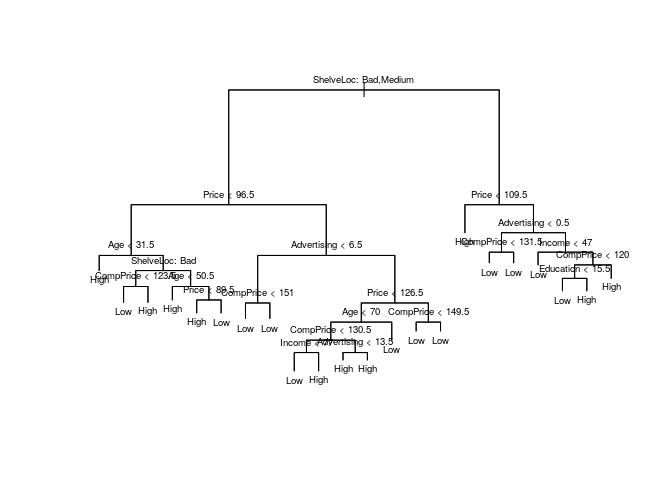
\includegraphics{02_Chi_Distrubition_files/figure-latex/unnamed-chunk-3-1.pdf}

\hypertarget{ggplot2}{%
\paragraph{GGPlot2}\label{ggplot2}}

\hypertarget{tidy-data}{%
\subparagraph{Tidy Data}\label{tidy-data}}

This can be done in ggplot2, but first a \texttt{tidy} data frame needs
to be constructed. Tidy data satisfies the following three rules:

\begin{enumerate}
\def\labelenumi{\arabic{enumi}.}
\tightlist
\item
  Each variable will have it's own column
\item
  Each ovservation will have it's own row
\item
  Each Value will have it's own cell.
\end{enumerate}

A tidy data frame somewhat depends on context, for example:

\begin{itemize}
\tightlist
\item
  If only the refugees were sampled, the data would be structured where:

  \begin{itemize}
  \tightlist
  \item
    Observations would be:

    \begin{itemize}
    \tightlist
    \item
      Low
    \item
      Medium
    \item
      High
    \end{itemize}
  \item
    Variables would be:

    \begin{itemize}
    \tightlist
    \item
      Count
    \end{itemize}
  \end{itemize}
\item
  If Multiple populations were sampled, for example the Australian
  population and the iraqi populations, the tidy data frame may be such
  that:

  \begin{itemize}
  \tightlist
  \item
    Observations would be:

    \begin{itemize}
    \tightlist
    \item
      Australia
    \item
      Iraqi
    \end{itemize}
  \item
    variables would be:

    \begin{itemize}
    \tightlist
    \item
      Count
    \item
      Distress Level
    \end{itemize}
  \end{itemize}
\item
  If Individuals were classified into a distress category, the
  corresponding tidy data frame would be:

  \begin{itemize}
  \tightlist
  \item
    Observations would be:

    \begin{itemize}
    \tightlist
    \item
      Individuals
    \end{itemize}
  \item
    variables would be:

    \begin{itemize}
    \tightlist
    \item
      Country of Origin/Residence
    \item
      Distress Level
    \end{itemize}
  \end{itemize}
\end{itemize}

\hypertarget{make-the-plot}{%
\subparagraph{Make the Plot}\label{make-the-plot}}

\begin{Shaded}
\begin{Highlighting}[]
\CommentTok{\#pivot\_longer(data = iraqi, cols = names(iraqi))}
\NormalTok{iraqi.tidy <{-}}\StringTok{ }\KeywordTok{melt}\NormalTok{(iraqi, }\DataTypeTok{value.name =} \StringTok{"Count"}\NormalTok{) }\OperatorTok{\%>\%}\StringTok{ }\KeywordTok{as\_tibble}\NormalTok{(}\DataTypeTok{rownames =} \StringTok{"Distress"}\NormalTok{)}
\NormalTok{iraqi.tidy}
\end{Highlighting}
\end{Shaded}

\begin{verbatim}
## # A tibble: 4 x 2
##   Distress Count
##   <chr>    <dbl>
## 1 low        123
## 2 moderate    70
## 3 high        93
## 4 veryHigh   157
\end{verbatim}

\begin{Shaded}
\begin{Highlighting}[]
\CommentTok{\# Base}
\CommentTok{\#barplot(height = iraqi.tidy$Count, names.arg = iraqi.tidy$Distress)}

\CommentTok{\# GGPlot2}
\KeywordTok{ggplot}\NormalTok{(}\DataTypeTok{data =}\NormalTok{ iraqi.tidy, }\DataTypeTok{mapping =} \KeywordTok{aes}\NormalTok{(}\DataTypeTok{x =}\NormalTok{ Distress, }\DataTypeTok{y =}\NormalTok{ Count)) }\OperatorTok{+}\StringTok{ }
\StringTok{  }\KeywordTok{geom\_col}\NormalTok{()}
\end{Highlighting}
\end{Shaded}

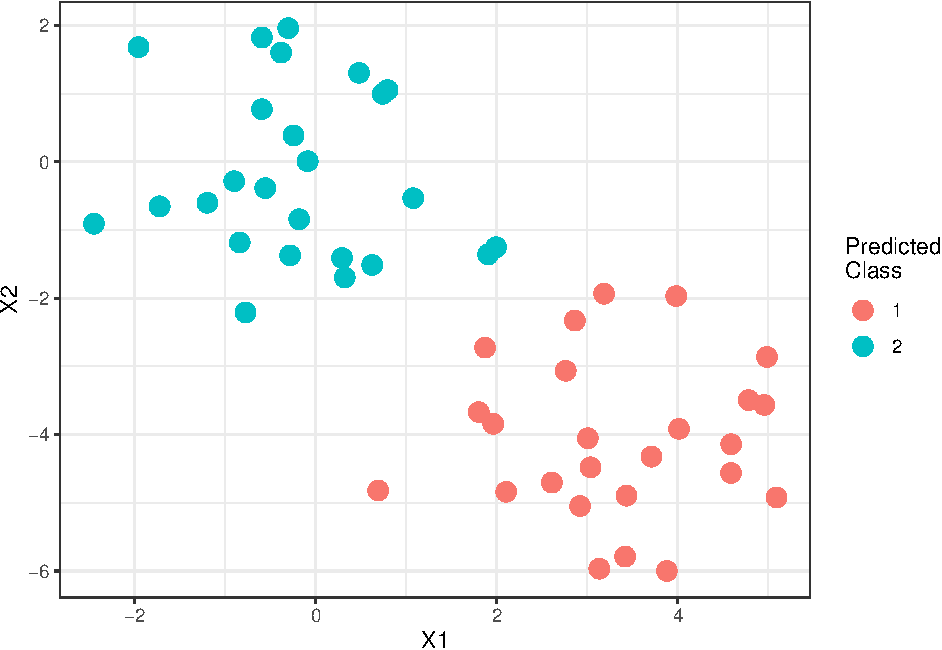
\includegraphics{02_Chi_Distrubition_files/figure-latex/unnamed-chunk-4-1.pdf}

\hypertarget{fix-the-order-of-the-plot}{%
\subparagraph{Fix the Order of the
Plot}\label{fix-the-order-of-the-plot}}

In making this plot you may observe that the order of the plot has been
made to be alphabetical, the order of the data frame has been
disregarded.

This is desirable and expected behaviour, the values of distress have
not been correctly encoded, they need to be encoded as ordered factors
in order to be ordered, unordered factors may as well be placed in
alphabetical order.

\begin{Shaded}
\begin{Highlighting}[]
\NormalTok{iraqi.tidy <{-}}\StringTok{ }\KeywordTok{melt}\NormalTok{(iraqi, }\DataTypeTok{value.name =} \StringTok{"Count"}\NormalTok{) }\OperatorTok{\%>\%}\StringTok{ }\KeywordTok{as\_tibble}\NormalTok{(}\DataTypeTok{rownames =} \StringTok{"Distress"}\NormalTok{)}
\NormalTok{iraqi.tidy}\OperatorTok{$}\NormalTok{Distress <{-}}\StringTok{ }\KeywordTok{factor}\NormalTok{(iraqi.tidy}\OperatorTok{$}\NormalTok{Distress, }\DataTypeTok{levels =}\NormalTok{ iraqi.tidy}\OperatorTok{$}\NormalTok{Distress, }\DataTypeTok{ordered =} \OtherTok{TRUE}\NormalTok{)}
\NormalTok{iraqi.tidy}
\end{Highlighting}
\end{Shaded}

\begin{verbatim}
## # A tibble: 4 x 2
##   Distress Count
##   <ord>    <dbl>
## 1 low        123
## 2 moderate    70
## 3 high        93
## 4 veryHigh   157
\end{verbatim}

\begin{Shaded}
\begin{Highlighting}[]
\CommentTok{\# Base}
\NormalTok{fillCols <{-}}\StringTok{ }\NormalTok{RColorBrewer}\OperatorTok{::}\KeywordTok{brewer.pal}\NormalTok{(}\KeywordTok{nrow}\NormalTok{(iraqi.tidy), }\DataTypeTok{name =} \StringTok{"Pastel1"}\NormalTok{)}
\KeywordTok{barplot}\NormalTok{(}\DataTypeTok{height =}\NormalTok{ iraqi.tidy}\OperatorTok{$}\NormalTok{Count, }\DataTypeTok{names.arg =} \KeywordTok{c}\NormalTok{(}\StringTok{"Low"}\NormalTok{, }\StringTok{"Moderate"}\NormalTok{, }\StringTok{"High"}\NormalTok{, }\StringTok{"Very High"}\NormalTok{), }\DataTypeTok{col =}\NormalTok{ fillCols, }\DataTypeTok{main =} \StringTok{"Distress Levels of Iraqi Refugees"}\NormalTok{, }\DataTypeTok{xlab =} \StringTok{"Distress Level"}\NormalTok{, }\DataTypeTok{ylab =} \StringTok{"Count"}\NormalTok{)}
\end{Highlighting}
\end{Shaded}

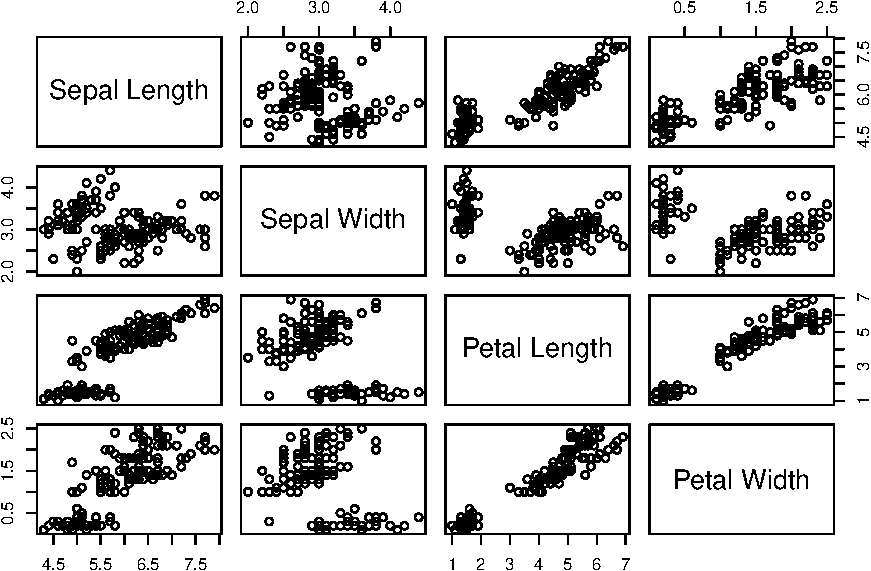
\includegraphics{02_Chi_Distrubition_files/figure-latex/unnamed-chunk-5-1.pdf}

\begin{Shaded}
\begin{Highlighting}[]
\CommentTok{\# GGPlot2}
\KeywordTok{ggplot}\NormalTok{(}\DataTypeTok{data =}\NormalTok{ iraqi.tidy, }\DataTypeTok{mapping =} \KeywordTok{aes}\NormalTok{(}\DataTypeTok{x =}\NormalTok{ Distress, }\DataTypeTok{y =}\NormalTok{ Count)) }\OperatorTok{+}\StringTok{ }
\StringTok{  }\KeywordTok{geom\_col}\NormalTok{(}\DataTypeTok{mapping =} \KeywordTok{aes}\NormalTok{(}\DataTypeTok{col =}\NormalTok{ Count, }\DataTypeTok{fill =}\NormalTok{ Distress)) }\OperatorTok{+}\StringTok{ }
\StringTok{  }\KeywordTok{theme\_classic}\NormalTok{() }\OperatorTok{+}
\StringTok{  }\KeywordTok{labs}\NormalTok{(}\DataTypeTok{title =} \StringTok{"Distress Levels of Iraqi Refugees"}\NormalTok{)}
\end{Highlighting}
\end{Shaded}

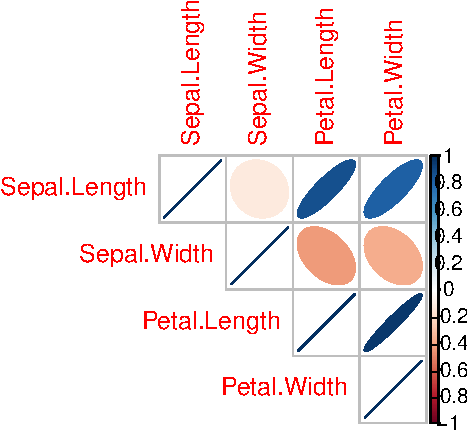
\includegraphics{02_Chi_Distrubition_files/figure-latex/unnamed-chunk-5-2.pdf}

\hypertarget{enter-the-aihw-data}{%
\subsubsection{(02) Enter the AIHW Data}\label{enter-the-aihw-data}}

The \emph{Australian Institute of Health and Wellness} data are as
follows:

\begin{Shaded}
\begin{Highlighting}[]
\NormalTok{aihw <{-}}\StringTok{ }\KeywordTok{c}\NormalTok{(}\StringTok{"low"}\NormalTok{ =}\StringTok{ }\FloatTok{70.65}\NormalTok{, }\StringTok{"moderate"}\NormalTok{ =}\StringTok{ }\FloatTok{18.5}\NormalTok{, }\StringTok{"high"}\NormalTok{ =}\StringTok{ }\FloatTok{7.41}\NormalTok{, }\StringTok{"veryHigh"}\NormalTok{ =}\StringTok{ }\FloatTok{3.43}\NormalTok{)}
\NormalTok{aihw.tidy <{-}}\StringTok{ }\NormalTok{tibble}\OperatorTok{::}\KeywordTok{enframe}\NormalTok{(aihw) }\CommentTok{\# \%>\% cbind(aihw, iraqi)}
\KeywordTok{names}\NormalTok{(aihw.tidy) <{-}}\StringTok{ }\KeywordTok{c}\NormalTok{(}\StringTok{"Distress"}\NormalTok{, }\StringTok{"Count"}\NormalTok{)}
\NormalTok{aihw.tidy}\OperatorTok{$}\NormalTok{Distress <{-}}\StringTok{ }\KeywordTok{factor}\NormalTok{(}\DataTypeTok{x =}\NormalTok{ aihw.tidy}\OperatorTok{$}\NormalTok{Distress, }\DataTypeTok{levels =}\NormalTok{ aihw.tidy}\OperatorTok{$}\NormalTok{Distress, }\DataTypeTok{ordered =} \OtherTok{TRUE}\NormalTok{)}
\NormalTok{aihw.tidy}
\end{Highlighting}
\end{Shaded}

\begin{verbatim}
## # A tibble: 4 x 2
##   Distress Count
##   <ord>    <dbl>
## 1 low      70.6 
## 2 moderate 18.5 
## 3 high      7.41
## 4 veryHigh  3.43
\end{verbatim}

\hypertarget{combine-all-observations}{%
\paragraph{Combine all Observations}\label{combine-all-observations}}

Ideally all the data should be combined into a single data set, be
mindful that \texttt{pivot\_longer()} is gonna complain if columns with
the same name have different data types, so make sure to remember to
re-class categories as factors rather than factors.:

\begin{Shaded}
\begin{Highlighting}[]
\CommentTok{\# First add a variable that can be used to distinguish the two Data Sets}
\NormalTok{iraqi.tidy}\OperatorTok{$}\NormalTok{Region <{-}}\StringTok{ "Iraq"}
\NormalTok{aihw.tidy}\OperatorTok{$}\NormalTok{Region <{-}}\StringTok{ "Australia"}
\CommentTok{\# Combine the Data Sets}
\NormalTok{all.tidy <{-}}\StringTok{ }\KeywordTok{rbind}\NormalTok{(iraqi.tidy, aihw.tidy) }
\NormalTok{all.tidy }
\end{Highlighting}
\end{Shaded}

\begin{verbatim}
## # A tibble: 8 x 3
##   Distress  Count Region   
##   <ord>     <dbl> <chr>    
## 1 low      123    Iraq     
## 2 moderate  70    Iraq     
## 3 high      93    Iraq     
## 4 veryHigh 157    Iraq     
## 5 low       70.6  Australia
## 6 moderate  18.5  Australia
## 7 high       7.41 Australia
## 8 veryHigh   3.43 Australia
\end{verbatim}

\begin{Shaded}
\begin{Highlighting}[]
\NormalTok{all.tidy}\OperatorTok{$}\NormalTok{Distress <{-}}\StringTok{ }\KeywordTok{factor}\NormalTok{(all.tidy}\OperatorTok{$}\NormalTok{Distress, }\DataTypeTok{levels =}\NormalTok{ iraqi.tidy}\OperatorTok{$}\NormalTok{Distress, }\DataTypeTok{ordered =} \OtherTok{TRUE}\NormalTok{)}

\CommentTok{\# Use Pivot Wider in order to make the column names the Region and the variable the count}
\NormalTok{all.wide <{-}}\StringTok{ }\KeywordTok{pivot\_wider}\NormalTok{(}\DataTypeTok{data =}\NormalTok{ all.tidy, }\DataTypeTok{names\_from =}\NormalTok{ Region, }\DataTypeTok{values\_from =}\NormalTok{ Count)}
\NormalTok{all.wide}
\end{Highlighting}
\end{Shaded}

\begin{verbatim}
## # A tibble: 4 x 3
##   Distress  Iraq Australia
##   <ord>    <dbl>     <dbl>
## 1 low        123     70.6 
## 2 moderate    70     18.5 
## 3 high        93      7.41
## 4 veryHigh   157      3.43
\end{verbatim}

\hypertarget{plot-the-aihw-data}{%
\paragraph{Plot the aihw Data}\label{plot-the-aihw-data}}

\begin{Shaded}
\begin{Highlighting}[]
\CommentTok{\# Base Plot}

\NormalTok{fillCols <{-}}\StringTok{ }\NormalTok{RColorBrewer}\OperatorTok{::}\KeywordTok{brewer.pal}\NormalTok{(}\KeywordTok{nrow}\NormalTok{(iraqi.tidy), }\DataTypeTok{name =} \StringTok{"Pastel2"}\NormalTok{)}
\KeywordTok{barplot}\NormalTok{(}\DataTypeTok{height =}\NormalTok{ all.wide}\OperatorTok{$}\NormalTok{Australia, }\DataTypeTok{names.arg =} \KeywordTok{c}\NormalTok{(}\StringTok{"Low"}\NormalTok{, }\StringTok{"Moderate"}\NormalTok{, }\StringTok{"High"}\NormalTok{, }\StringTok{"Very High"}\NormalTok{), }\DataTypeTok{col =}\NormalTok{ fillCols, }\DataTypeTok{main =} \StringTok{"Distress Levels of Iraqi Refugees"}\NormalTok{, }\DataTypeTok{xlab =} \StringTok{"Distress Level"}\NormalTok{, }\DataTypeTok{ylab =} \StringTok{"Count"}\NormalTok{)}
\end{Highlighting}
\end{Shaded}

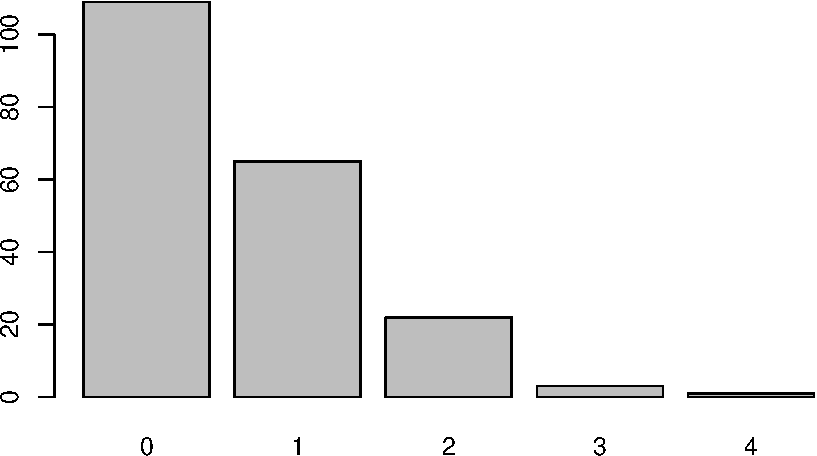
\includegraphics{02_Chi_Distrubition_files/figure-latex/unnamed-chunk-8-1.pdf}

\begin{Shaded}
\begin{Highlighting}[]
\CommentTok{\#\# ggplot2}
\KeywordTok{ggplot}\NormalTok{(}\DataTypeTok{data =}\NormalTok{ all.tidy, }\DataTypeTok{mapping =} \KeywordTok{aes}\NormalTok{(}\DataTypeTok{x =}\NormalTok{ Distress, }\DataTypeTok{y =}\NormalTok{ Count, }\DataTypeTok{fill =}\NormalTok{ Region, }\DataTypeTok{col =}\NormalTok{ Count)) }\OperatorTok{+}
\StringTok{  }\KeywordTok{geom\_col}\NormalTok{(}\DataTypeTok{position =} \StringTok{"dodge"}\NormalTok{) }\OperatorTok{+}
\StringTok{  }\KeywordTok{guides}\NormalTok{(}\DataTypeTok{col =} \OtherTok{FALSE}\NormalTok{) }\OperatorTok{+}
\StringTok{  }\KeywordTok{theme\_classic}\NormalTok{() }\OperatorTok{+}
\StringTok{  }\KeywordTok{labs}\NormalTok{(}\DataTypeTok{title =} \StringTok{"Distress of Refugees"}\NormalTok{, }\DataTypeTok{subtitle =} \StringTok{""}\NormalTok{, }\DataTypeTok{y =} \StringTok{"Frequency"}\NormalTok{)}
\end{Highlighting}
\end{Shaded}

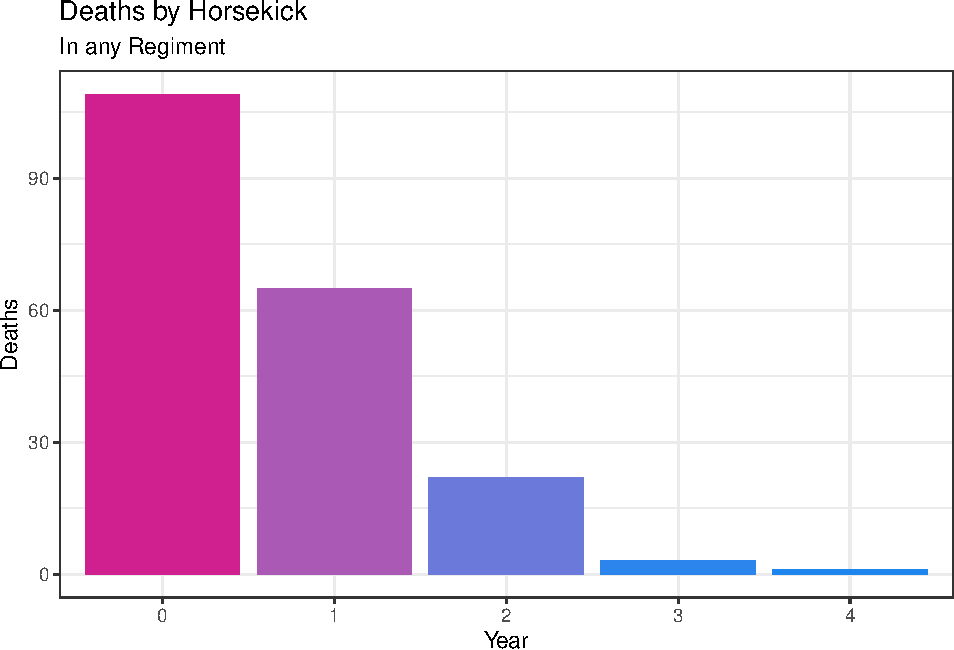
\includegraphics{02_Chi_Distrubition_files/figure-latex/unnamed-chunk-8-2.pdf}

\hypertarget{determine-expected-frequency}{%
\subsubsection{(03) Determine Expected
Frequency}\label{determine-expected-frequency}}

\hypertarget{hypothesis}{%
\paragraph{Hypothesis}\label{hypothesis}}

\begin{enumerate}
\def\labelenumi{\arabic{enumi}.}
\tightlist
\item
  \(H_0 \enspace : \quad\) The Refugee Distress Categories will have
  frequencies equal to Australia
\item
  \(H_a \enspace : \quad\) There will be a difference between the
  categories
\end{enumerate}

Assuming that the null hypothesis is true, the expected frequency of the
categories can be deterimed:

\[
\textsf{e} = 443 \times \frac{\verb| aihw |}{100}
\]

\begin{Shaded}
\begin{Highlighting}[]
\NormalTok{all.wide}\OperatorTok{$}\NormalTok{IraqExpected <{-}}\StringTok{ }\NormalTok{all.wide}\OperatorTok{$}\NormalTok{Australia }\OperatorTok{*}\StringTok{ }\NormalTok{(}\KeywordTok{sum}\NormalTok{(all.wide}\OperatorTok{$}\NormalTok{Iraq)}\OperatorTok{/}\DecValTok{100}\NormalTok{)}

\CommentTok{\# Rename the Column to reflect expected and observed frequencies}

\CommentTok{\#\# using Dplyer}
\NormalTok{all.wide }\OperatorTok{\%>\%}\StringTok{ }
\StringTok{  }\NormalTok{dplyr}\OperatorTok{::}\KeywordTok{rename}\NormalTok{(}
    \DataTypeTok{IraqObserved =}\NormalTok{ Iraq}
\NormalTok{  )}
\end{Highlighting}
\end{Shaded}

\begin{verbatim}
## # A tibble: 4 x 4
##   Distress IraqObserved Australia IraqExpected
##   <ord>           <dbl>     <dbl>        <dbl>
## 1 low               123     70.6         313. 
## 2 moderate           70     18.5          82.0
## 3 high               93      7.41         32.8
## 4 veryHigh          157      3.43         15.2
\end{verbatim}

\begin{Shaded}
\begin{Highlighting}[]
\CommentTok{\#\# using Base Functions}
\KeywordTok{names}\NormalTok{(all.wide)[}\KeywordTok{names}\NormalTok{(all.wide)}\OperatorTok{==}\StringTok{"Iraq"}\NormalTok{] <{-}}\StringTok{ "IraqObserved"}

\CommentTok{\# Print the DataFrame}
\NormalTok{all.wide}
\end{Highlighting}
\end{Shaded}

\begin{verbatim}
## # A tibble: 4 x 4
##   Distress IraqObserved Australia IraqExpected
##   <ord>           <dbl>     <dbl>        <dbl>
## 1 low               123     70.6         313. 
## 2 moderate           70     18.5          82.0
## 3 high               93      7.41         32.8
## 4 veryHigh          157      3.43         15.2
\end{verbatim}

\hypertarget{compute-the-chi-squared-distance}{%
\subsubsection{(04)Compute the Chi-Squared
Distance}\label{compute-the-chi-squared-distance}}

The \emph{Chi-Squared} (\(\chi^2\)) statistic is the squared distance
from the the expected and observed values to the expected value:

\[
\chi^2 = \sum^n_{i=1} \left[ \frac{(o-e)^2}{e} \right]
\]

This can be done readily in \textbf{\emph{R}}:

\begin{Shaded}
\begin{Highlighting}[]
\NormalTok{o <{-}}\StringTok{ }\NormalTok{all.wide}\OperatorTok{$}\NormalTok{IraqObserved}
\NormalTok{e <{-}}\StringTok{ }\NormalTok{all.wide}\OperatorTok{$}\NormalTok{IraqExpected}

\NormalTok{all.wide}\OperatorTok{$}\NormalTok{ChiDist <{-}}\StringTok{ }\NormalTok{((o}\OperatorTok{{-}}\NormalTok{e)}\OperatorTok{\^{}}\DecValTok{2}\OperatorTok{/}\NormalTok{e)}
\NormalTok{ChiStat <{-}}\StringTok{ }\KeywordTok{sum}\NormalTok{(all.wide}\OperatorTok{$}\NormalTok{ChiDist)}
\NormalTok{ChiStat}
\end{Highlighting}
\end{Shaded}

\begin{verbatim}
## [1] 1550.75
\end{verbatim}

And returns the value \(\chi^2 \approx 1551\)

\hypertarget{similate-the-counts}{%
\subsubsection{(05) Similate the Counts}\label{similate-the-counts}}

A distribution with multiple categories of different probabilities is a
\textbf{multinomial} distribution and can be simulated:

\begin{Shaded}
\begin{Highlighting}[]
\KeywordTok{rmultinom}\NormalTok{(}\DataTypeTok{n =} \DecValTok{1}\NormalTok{, }\DataTypeTok{size =} \DecValTok{443}\NormalTok{, }\DataTypeTok{prob =}\NormalTok{ aihw}\OperatorTok{/}\DecValTok{100}\NormalTok{)}
\end{Highlighting}
\end{Shaded}

\begin{verbatim}
##          [,1]
## low       311
## moderate   74
## high       34
## veryHigh   24
\end{verbatim}

\begin{Shaded}
\begin{Highlighting}[]
\CommentTok{\# A more Rigurous simulation by averaging various other simulations}
\NormalTok{average\_sim\_count      <{-}}\StringTok{ }\KeywordTok{rmultinom}\NormalTok{(}\DataTypeTok{n =} \DecValTok{10000}\NormalTok{, }\DataTypeTok{size =} \DecValTok{443}\NormalTok{, }\DataTypeTok{prob =}\NormalTok{ aihw}\OperatorTok{/}\DecValTok{100}\NormalTok{) }\OperatorTok{\%>\%}\StringTok{ }\KeywordTok{rowMeans}\NormalTok{()}
\NormalTok{all.wide}\OperatorTok{$}\NormalTok{IraqSimulated <{-}}\StringTok{ }\NormalTok{average\_sim\_count }
\NormalTok{all.wide}
\end{Highlighting}
\end{Shaded}

\begin{verbatim}
## # A tibble: 4 x 6
##   Distress IraqObserved Australia IraqExpected ChiDist IraqSimulated
##   <ord>           <dbl>     <dbl>        <dbl>   <dbl>         <dbl>
## 1 low               123     70.6         313.   115.           313. 
## 2 moderate           70     18.5          82.0    1.74          81.9
## 3 high               93      7.41         32.8  110.            32.9
## 4 veryHigh          157      3.43         15.2 1323.            15.2
\end{verbatim}

\begin{Shaded}
\begin{Highlighting}[]
\CommentTok{\# Building a Confidence Interval for the true mean given this Distribution}
\CommentTok{\# The confidence interval is meaningless really, it can be made arbitrarily small by}
\CommentTok{\# making n sufficietnly large, this is just to illustrate confidence intervals for}
\CommentTok{\# population means given a sample of sample means.}
\NormalTok{sd\_sim\_count      <{-}}\StringTok{ }\KeywordTok{rmultinom}\NormalTok{(}\DataTypeTok{n =} \DecValTok{1000}\NormalTok{, }\DataTypeTok{size =} \DecValTok{443}\NormalTok{, }\DataTypeTok{prob =}\NormalTok{ aihw}\OperatorTok{/}\DecValTok{100}\NormalTok{) }\OperatorTok{\%>\%}\StringTok{ }\KeywordTok{apply}\NormalTok{(}\DataTypeTok{MARGIN =} \DecValTok{1}\NormalTok{, sd) }\CommentTok{\# 1 is row, 2 is column}

\CommentTok{\# Calculate the t{-}statistic for 95\%}
\NormalTok{t <{-}}\StringTok{ }\KeywordTok{qt}\NormalTok{(}\DataTypeTok{p =} \FloatTok{0.95}\NormalTok{, }\DataTypeTok{df =} \DecValTok{999}\NormalTok{)}

\KeywordTok{data.frame}\NormalTok{(}
  \DataTypeTok{averageSimCount =}\NormalTok{ average\_sim\_count,}
  \DataTypeTok{sdSimCount =}\NormalTok{ sd\_sim\_count,}
  \DataTypeTok{lowerConfidenceForMean=} \KeywordTok{round}\NormalTok{(average\_sim\_count }\OperatorTok{{-}}\StringTok{ }\NormalTok{t }\OperatorTok{*}\StringTok{ }\NormalTok{(sd\_sim\_count)}\OperatorTok{/}\KeywordTok{sqrt}\NormalTok{(}\DecValTok{1000}\NormalTok{)),}
  \DataTypeTok{upperConfidenceForMean =} \KeywordTok{round}\NormalTok{(average\_sim\_count }\OperatorTok{+}\StringTok{ }\NormalTok{t }\OperatorTok{*}\StringTok{ }\NormalTok{(sd\_sim\_count)}\OperatorTok{/}\KeywordTok{sqrt}\NormalTok{(}\DecValTok{1000}\NormalTok{))}
\NormalTok{)}
\end{Highlighting}
\end{Shaded}

\begin{verbatim}
##          averageSimCount sdSimCount lowerConfidenceForMean
## low             313.0281   9.650622                    313
## moderate         81.9252   8.238560                     81
## high             32.8949   5.338517                     33
## veryHigh         15.1518   3.839398                     15
##          upperConfidenceForMean
## low                         314
## moderate                     82
## high                         33
## veryHigh                     15
\end{verbatim}

Or this could be simulated by using the \texttt{sample()} function:

\begin{Shaded}
\begin{Highlighting}[]
\NormalTok{frequency <{-}}\StringTok{ }\KeywordTok{sample}\NormalTok{(}\DecValTok{1}\OperatorTok{:}\DecValTok{4}\NormalTok{, }\DecValTok{443}\NormalTok{, }\DataTypeTok{replace =} \OtherTok{TRUE}\NormalTok{, }\DataTypeTok{prob=}\NormalTok{all.wide}\OperatorTok{$}\NormalTok{Australia) }\OperatorTok{\%>\%}
\StringTok{  }\NormalTok{table }\OperatorTok{\%>\%}\StringTok{ }
\StringTok{  }\NormalTok{tibble}\OperatorTok{::}\KeywordTok{enframe}\NormalTok{()}

\KeywordTok{names}\NormalTok{(frequency) <{-}}\StringTok{ }\KeywordTok{c}\NormalTok{(}\StringTok{"Distress"}\NormalTok{, }\StringTok{"Count"}\NormalTok{)}
\NormalTok{frequency}\OperatorTok{$}\NormalTok{Distress <{-}}\StringTok{ }\KeywordTok{names}\NormalTok{(iraqi)}
\NormalTok{frequency}
\end{Highlighting}
\end{Shaded}

\begin{verbatim}
## # A tibble: 4 x 2
##   Distress Count  
##   <chr>    <table>
## 1 low      315    
## 2 moderate  88    
## 3 high      26    
## 4 veryHigh  14
\end{verbatim}

\hypertarget{put-everything-together}{%
\subsubsection{(06) Put Everything
together}\label{put-everything-together}}

So the idea is, in order to test the hypothesis that there is no
difference we will set up a hypothesis test.

The test statistic will be the total squared distance relative to the
expected value for the distribution, this is known as the \(\chi ^2\)
value.

If we can:

\begin{itemize}
\tightlist
\item
  Assume the null hypothesis is true

  \begin{itemize}
  \tightlist
  \item
    (no difference between the number of iraqi counts and the number of
    \texttt{aihw} counts)
  \end{itemize}
\item
  With only 5\% probability of getting a false positive under this
  assumption
\end{itemize}

then we will reject the null hypothesis that they are the same and
accept that there is a significant difference between the distribution
of distress in the iraqi population. + (this necessarily show that the
iraqi refugees are more distressed, merely that the distribution is
different from the Australian distribution in such a way that would be
unlikely to be a false positive assuming they were identical.)

In order to evaluate this, We can take a random sample of values that
are distributed with the same frequency as the \texttt{aihw} data and
measure how often the corresponding \(\chi^2\) value of the sampled
values exceed that of the observed values for the iraqi values, under
the assumption that the iraqi values are distributed at the same
frequency of the \texttt{aihw}, this would amount to a False Positive
for a difference.

Creating many chi statistics, comparing them and repeating gives a false
positive rate:

\begin{Shaded}
\begin{Highlighting}[]
\CommentTok{\# Calcualate the iraqi Chi Stat}
\NormalTok{e <{-}}\StringTok{ }\NormalTok{aihw}\OperatorTok{/}\DecValTok{100} \OperatorTok{*}\StringTok{ }\KeywordTok{sum}\NormalTok{(iraqi)}
\NormalTok{o <{-}}\StringTok{ }\NormalTok{iraqi}
\NormalTok{iraqi\_chi <{-}}\StringTok{ }\KeywordTok{sum}\NormalTok{((e}\OperatorTok{{-}}\NormalTok{o)}\OperatorTok{\^{}}\DecValTok{2}\OperatorTok{/}\NormalTok{e)}

\CommentTok{\# Simulate the False Positive Rate for data following the Aus Distribution}
\NormalTok{n <{-}}\StringTok{ }\DecValTok{10}\OperatorTok{\^{}}\DecValTok{3} \CommentTok{\# Simulation Length}
\NormalTok{FalsePosVec <{-}}\StringTok{ }\KeywordTok{vector}\NormalTok{(}\DataTypeTok{length =}\NormalTok{ n)}
\ControlFlowTok{for}\NormalTok{ (i }\ControlFlowTok{in} \DecValTok{1}\OperatorTok{:}\NormalTok{n) \{}
 \CommentTok{\# e <{-} rmultinom(1, 443, aihw/100)}
\NormalTok{  e <{-}}\StringTok{  }\KeywordTok{sample}\NormalTok{(}\DecValTok{1}\OperatorTok{:}\DecValTok{4}\NormalTok{, }\DecValTok{443}\NormalTok{, }\DataTypeTok{replace =} \OtherTok{TRUE}\NormalTok{, }\DataTypeTok{prob=}\NormalTok{aihw) }\OperatorTok{\%>\%}\StringTok{  }\NormalTok{table}
\NormalTok{  o <{-}}\StringTok{ }\NormalTok{aihw}
\CommentTok{\#  o <{-} iraqi}
\NormalTok{  sim\_chi <{-}}\StringTok{ }\KeywordTok{sum}\NormalTok{((e}\OperatorTok{{-}}\NormalTok{o)}\OperatorTok{\^{}}\DecValTok{2}\OperatorTok{/}\NormalTok{e )}
  \CommentTok{\# Assume null hypotheses, this means we assume the iraqi distance does not exceed the sim distance}
  \CommentTok{\# The number of times it does exceed is:}
      \CommentTok{\# the probability of a false positive assuming the null hypothesis is correct}
           \CommentTok{\# this is the p{-}value.}
\NormalTok{  FalsePosQ <{-}}\StringTok{ }\OperatorTok{!}\NormalTok{(iraqi\_chi }\OperatorTok{<}\StringTok{ }\NormalTok{sim\_chi) }\CommentTok{\#(assuming null hypothesis means assuming iraqi distance leq to  sim)}
                                     \CommentTok{\# The number of positives will be the FPR and indicative of }
                                     \CommentTok{\# the p{-}value)}
\NormalTok{  FalsePosVec[i] <{-}}\StringTok{ }\NormalTok{FalsePosQ}
\NormalTok{\}}

\NormalTok{pval <{-}}\StringTok{ }\KeywordTok{mean}\NormalTok{(FalsePosVec)}
\KeywordTok{print}\NormalTok{(pval)}
\end{Highlighting}
\end{Shaded}

\begin{verbatim}
## [1] 1
\end{verbatim}

This could be made more efficient by using \texttt{replicate} rather
than a \texttt{for} loop (\texttt{replicate} is to \textbf{\emph{R}} as
\texttt{Table{[}{]}} is to \emph{Mathematica}):

\begin{Shaded}
\begin{Highlighting}[]
\NormalTok{e <{-}}\StringTok{ }\NormalTok{aihw}\OperatorTok{/}\DecValTok{100} \OperatorTok{*}\StringTok{ }\KeywordTok{sum}\NormalTok{(iraqi)}
\NormalTok{o <{-}}\StringTok{ }\NormalTok{iraqi}
\NormalTok{iraqi\_chi <{-}}\StringTok{ }\KeywordTok{sum}\NormalTok{((e}\OperatorTok{{-}}\NormalTok{o)}\OperatorTok{\^{}}\DecValTok{2}\OperatorTok{/}\NormalTok{e)}

\NormalTok{FalsePosCount <{-}}\StringTok{ }\KeywordTok{replicate}\NormalTok{(}\DecValTok{10}\OperatorTok{\^{}}\DecValTok{4}\NormalTok{, }\DataTypeTok{expr =}\NormalTok{ \{}
\NormalTok{  o <{-}}\StringTok{ }\KeywordTok{rmultinom}\NormalTok{(}\DataTypeTok{n =} \DecValTok{1}\NormalTok{, }\DataTypeTok{size =} \KeywordTok{sum}\NormalTok{(iraqi), }\DataTypeTok{prob =}\NormalTok{ aihw)}
\NormalTok{  sim\_chi <{-}}\StringTok{ }\KeywordTok{sum}\NormalTok{((e}\OperatorTok{{-}}\NormalTok{o)}\OperatorTok{\^{}}\DecValTok{2}\OperatorTok{/}\NormalTok{e)}
  \OperatorTok{!}\NormalTok{(iraqi\_chi }\OperatorTok{<}\StringTok{ }\NormalTok{sim\_chi)}
\NormalTok{\})}

\KeywordTok{mean}\NormalTok{(FalsePosCount)}
\end{Highlighting}
\end{Shaded}

\begin{verbatim}
## [1] 1
\end{verbatim}

This returns a value of 1, indicating that the probability of a false
positive, assuming that the data was randomly sampled following the
probabilities of the proportions of the Australian populatation, is
effectively 1, thus the null hypothesis should be rejected and the
alternative hypothesis accepted.

\hypertarget{use-the-inbuilt-chi-square-statistic}{%
\subsubsection{(07) Use the InBuilt Chi-Square
Statistic}\label{use-the-inbuilt-chi-square-statistic}}

The chi-squared value that would correspond to a false positive rate
like in the above simulation, may be determined by integrating the
appropriate probability density function:

\[
\begin{aligned}
f_n\left( x \right)= \frac{1}{2^{\frac{n}{2}} \cdot  \Gamma\left( \frac{n}{2} \right)} \cdot  x^{\frac{n}{2} -  1}\cdot  e^{- \frac{x}{2}}
\end{aligned}
\]

where the mean and variance are \(n\) and \(2n\) respectively;
\(\Gamma\left( x \right)\) is the gamma function it's very similar to
the factorial function (\(x!\)):

\[\begin{aligned}
x! &= \Gamma\left( x+ 1 \right)\\
x! &= x \cdot  \Gamma\left( x \right)\\
\Gamma\left( n \right)&= \left( n- 1 \right)!, \qquad \forall n \in \mathbb{Z} \setminus \mathbb{Z}^- \\
\Gamma\left( z \right) &= \int_{0}^{\infty}\left(  \left( \# \right)^{z- 1}\cdot  e^{-\left( \# \right)} \right) \mathrm{d} \left( \# \right), \qquad z \in \mathbb{C} \wedge \Re\left( z \right)>0
\end{aligned}\]

This doesn't seem quick to solve, plugging it into \emph{Mathematica}
gives:

\begin{verbatim}
Integrate[ 1/2^(n/2*Gamma[n/2])*x^(n/2 - 1)*e^(-x/2), {x, 0, \[Infinity]}]
\end{verbatim}

\begin{verbatim}
ConditionalExpression[(2^(1/2 - (3 Sqrt[\[Pi]])/4) Sqrt[\[Pi]])/ Log[e]^(3/2), Re[Log[e]] > 0]
\end{verbatim}

\[
\int^{\infty}_0\frac{1}{2^{\frac{n}{2}} \cdot  \Gamma\left( \frac{n}{2} \right)} \cdot  x^{\frac{n}{2} -  1}\cdot  e^{- \frac{x}{2}} \enspace \mathrm{d}x =   \frac{2^{\frac{1}{2}-\frac{3 \sqrt{\pi }}{4}} \sqrt{\pi }}{\log ^{\frac{3}{2}}(e)} 
 \]

Howerver inside \textbf{\emph{R}} this is all built into the
\texttt{pchisq()} function and the null hypothesis may be evaluated
without necessarily undertaking the simulation.

\hypertarget{evaluate-test-statistic-using-chi-statistic}{%
\paragraph{Evaluate Test Statistic Using Chi
Statistic}\label{evaluate-test-statistic-using-chi-statistic}}

The probability of a false positive, assuming that the null hypothesis
is true can be determined directly from the critical values of the
Chi-Statistic.

\begin{Shaded}
\begin{Highlighting}[]
\CommentTok{\# the null hypothesis is that there is no difference, the}
\CommentTok{\# probability of detecting a difference will be the upper tail and would be the p{-}value}
\KeywordTok{pchisq}\NormalTok{(}\DataTypeTok{q =}\NormalTok{ iraqi\_chi, }\DataTypeTok{df =}\NormalTok{ (}\KeywordTok{length}\NormalTok{(aihw)}\OperatorTok{{-}}\DecValTok{1}\NormalTok{), }\DataTypeTok{lower.tail =} \OtherTok{FALSE}\NormalTok{)}
\end{Highlighting}
\end{Shaded}

\begin{verbatim}
## [1] 0
\end{verbatim}

It isn't even necessary to calculate the \(\chi^2\) value, this is built
into \textbf{\emph{R}} and can be done all at once:

\begin{Shaded}
\begin{Highlighting}[]
\KeywordTok{chisq.test}\NormalTok{(}\DataTypeTok{x =}\NormalTok{ iraqi, }\DataTypeTok{p =}\NormalTok{ aihw, }\DataTypeTok{rescale.p =} \OtherTok{TRUE}\NormalTok{)}
\end{Highlighting}
\end{Shaded}

\begin{verbatim}
## 
##  Chi-squared test for given probabilities
## 
## data:  iraqi
## X-squared = 1550.6, df = 3, p-value < 2.2e-16
\end{verbatim}

As opposed to using the \(\chi^2\) distribution, it is possible to use a
\emph{Monte Carlo} simulation all in one line as well:

\begin{Shaded}
\begin{Highlighting}[]
\KeywordTok{chisq.test}\NormalTok{(}\DataTypeTok{x =}\NormalTok{ iraqi, }\DataTypeTok{p =}\NormalTok{ aihw, }\DataTypeTok{rescale.p =} \OtherTok{TRUE}\NormalTok{, }\DataTypeTok{simulate.p.value =} \OtherTok{TRUE}\NormalTok{, }\DataTypeTok{B =} \DecValTok{10}\OperatorTok{\^{}}\DecValTok{3}\NormalTok{)}
\end{Highlighting}
\end{Shaded}

\begin{verbatim}
## 
##  Chi-squared test for given probabilities with simulated p-value (based
##  on 1000 replicates)
## 
## data:  iraqi
## X-squared = 1550.6, df = NA, p-value = 0.000999
\end{verbatim}

I can't think of any reason to use the monte carlo simulation over the
density distribution though

\hypertarget{eels-data-comparison-of-two-populations}{%
\subsection{Eels Data (Comparison of Two
Populations)}\label{eels-data-comparison-of-two-populations}}

\hypertarget{enter-the-data}{%
\subsubsection{(1) Enter the Data}\label{enter-the-data}}

\hypertarget{expected-values}{%
\subsubsection{(2) Expected Values}\label{expected-values}}

\hypertarget{simulate-the-values}{%
\subsubsection{(3) Simulate The Values}\label{simulate-the-values}}

\hypertarget{use-the-chi-squared-distribution}{%
\subsubsection{(4) Use the Chi Squared
Distribution}\label{use-the-chi-squared-distribution}}

\hypertarget{other-examples}{%
\subsection{Other Examples}\label{other-examples}}

\hypertarget{daily-frequency}{%
\subsubsection{(1) Daily Frequency}\label{daily-frequency}}

\hypertarget{mendellian-genetics}{%
\subsubsection{(2) Mendellian Genetics}\label{mendellian-genetics}}

\hypertarget{political-opinion}{%
\subsubsection{(3) Political Opinion}\label{political-opinion}}

\hypertarget{medical-efficacy}{%
\subsubsection{(4) Medical Efficacy}\label{medical-efficacy}}

\end{document}
